% Copyright 2004 by Till Tantau <tantau@users.sourceforge.net>.
%
% In principle, this file can be redistributed and/or modified under
% the terms of the GNU Public License, version 2.
%
% However, this file is supposed to be a template to be modified
% for your own needs. For this reason, if you use this file as a
% template and not specifically distribute it as part of a another
% package/program, I grant the extra permission to freely copy and
% modify this file as you see fit and even to delete this copyright
% notice. 

\documentclass{beamer}
% Replace the \documentclass declaration above
% with the following two lines to typeset your 
% lecture notes as a handout:
%\documentclass{article}
%\usepackage{beamerarticle}


% There are many different themes available for Beamer. A comprehensive
% list with examples is given here:
% http://deic.uab.es/~iblanes/beamer_gallery/index_by_theme.html
% You can uncomment the themes below if you would like to use a different
% one:
%\usetheme{AnnArbor}
%\usetheme{Antibes}
%\usetheme{Bergen}
% \usetheme{Berkeley}
% \usetheme{Berlin}
% \usetheme{Boadilla}
%\usetheme{boxes}
% \usetheme{CambridgeUS}
% \usetheme{Copenhagen}
%\usetheme{Darmstadt}
%\usetheme{default}
%\usetheme{Frankfurt}
% \usetheme{Goettingen}
% \usetheme{Hannover}
%\usetheme{Ilmenau}
%\usetheme{JuanLesPins}
\usetheme{Luebeck}
% \usetheme{Madrid}
%\usetheme{Malmoe}
% \usetheme{Marburg}
% \usetheme{Montpellier}
% \usetheme{PaloAlto}
%\usetheme{Pittsburgh}
%\usetheme{Rochester}
%\usetheme{Singapore}
%\usetheme{Szeged}
% \usetheme{Warsaw}
\usepackage{multicol}
\usepackage{xcolor}
\usepackage{hyperref}
\usepackage{graphicx}
\usepackage{wrapfig}
\usepackage{braket}
\usepackage{bigints}
\usepackage{amsmath}
\usepackage{amssymb}
\usepackage{amsthm}
\usepackage{bm}
% \AtBeginSubsection[]
% {
%   \begin{frame}<beamer>
%    \begin{multicols}{2}
%      \tableofcontents[currentsection,hideothersubsection]
%    \end{multicols}
%   \end{frame}
% }

% \usecolortheme{structure}

\graphicspath{{./images/},{./figures/}}

\title{Periodically Driven Aubry-Andr\'{e}-Harper Models}

% A subtitle is optional and this may be deleted
% \subtitle{Optional Subtitle}

\author{\href{mailto:rajath.shashidhara@gmail.com}{Rajath S} \\ \texttt{2012B5A7589P}}
% - Give the names in the same order as the appear in the paper.
% - Use the \inst{?} command only if the authors have different
%   affiliation.

\institute[Birla Institute of Technology and Science, Pilani] % (optional, but mostly needed)
{
  \tiny Under the supervision of \\  
  \normalsize Dr. Tapomoy Guha Sarkar\\ 
  \footnotesize Department of Physics\\
  Birla Institute of Technology and Science, Pilani\\ \normalsize
  
\includegraphics[width=0.15\textwidth]{logo.png}\\
  }
%   \and
%   \inst{2}%
%   Department of Theoretical Philosophy\\
%   University of Elsewhere}
% - Use the \inst command only if there are several affiliations.
% - Keep it simple, no one is interested in your street address.

% \date{Conference Name, 2013}
% - Either use conference name or its abbreviation.
% - Not really informative to the audience, more for people (including
%   yourself) who are reading the slides online

\subject{Condensed Matter Physics}
% This is only inserted into the PDF information catalog. Can be left
% out. 

% If you have a file called "university-logo-filename.xxx", where xxx
% is a graphic format that can be processed by latex or pdflatex,
% resp., then you can add a logo as follows:
% \pgfdeclareimage[height=0.5cm]{university-logo}{images/logo}
% \logo{\pgfuseimage{university-logo}}

% Delete this, if you do not want the table of contents to pop up at
% the beginning of each subsection:
% \AtBeginSubsection[]
% {
%   \begin{frame}<beamer>{Outline}
%     \tableofcontents[currentsection,currentsubsection]
%   \end{frame}
% }

% Let's get started
\begin{document}

\begin{frame}
  \titlepage
\end{frame}

\begin{frame}{Introduction}
  \begin{multicols}{2}
    \tableofcontents
  \end{multicols}
  % You might wish to add the option [pausesections]
\end{frame}

% Section and subsections will appear in the presentation overview
% and table of contents.
\section{Geometric Phase}

\subsection{Berry's discovery}

\begin{frame}{Berry's Discovery}{Cyclic Adiabatic evolution}
  \begin{itemize}
  \item {
    Gauge freedom in Quantum Mechanics.
  }
  \item {
    Parameter space $\mathbf{R}$ and Vector line bundle $\ket{n(\mathbf{R})}$.
  }
  \item{
    Single-valued Eigenvectors in Parameter space.
  }
  \item {
    Assumptions : Adiabatic evolution, No degeneracies/level crossings, Schrodinger evolution
  }  
  \end{itemize}  
  Expand as \begin{equation*}
             \ket{\psi(t)} = \sum{c_{n}(t) e^{-\frac{i}{\hbar}\int_{0}^{t}{E_{n}(t) dt}} \ket{n(t)}}
            \end{equation*}
  If at $t=0$, $\ket{\psi(0)} = \ket{n(0)}$, from time-dependent perturbation theory
  \begin{equation*}
    \ket{\psi(T)} = e^{i \gamma_{n}(T)} e^{i \theta_{n}(T)} \ket{\psi(0)}
  \end{equation*} (Quantum Adiabatic Theorem)
\end{frame}

\begin{frame}{Geometric properties}
From adiabatic theorem
    \begin{equation*}
     \gamma_{n}(T) = i\,\int_{0}^{T}{\braket{n(t) | \frac{\partial}{\partial t} n(t)}\, dt} = i\, \oint_{c}{\braket{n(\mathbf{R})| \bm{\nabla_{R}} | n(\mathbf{R})} \cdot \, d\mathbf{R}}
    \end{equation*}
    By Stokes theorem,
    \small\begin{equation*}
     \gamma_{n}(T) = i \bigintsss_{S}{\,\sum_{m \neq n}{\frac{\braket{n(\mathbf{R})|\bm{\nabla_{R}}\hat{H}(\mathbf{R})|m(\mathbf{R})} \wedge \braket{m(\mathbf{R})|\bm{\nabla_{R}}\hat{H}(\mathbf{R})|n(\mathbf{R})}}{(E_{n}(\mathbf{R})- E_{m}(\mathbf{R}))^2}} \cdot \, d\mathbf{S}}
    \end{equation*}\normalsize
  \begin{itemize}
  \item{
    Path-integral. Gauge Invariant. Reparameterization invariant.
  }
  \item {
    Not single-valued on parameter space $\implies$ Non-integrable; Cannot be expressed as a scalar field over parameter space.
  }
  \item {
    Physically observable. (Aharanov-Bohm effect)
  }
  \item {
    Analogy to Parallel transport of vectors on curved manifold.
  }
  \end{itemize}
\end{frame}

\begin{frame}{Analogy to Electromagnetism}
\begin{block}{Berry Connection}
\begin{equation}
 \mathbf{A}_{n}(\mathbf{R}) = i\braket{n(\mathbf{R})| \bm{\nabla_{R}} | n(\mathbf{R})}
\end{equation}
\end{block}
\begin{block}{Berry Curvature}
\begin{equation}
 \mathbf{B}_{n}(\mathbf{R}) = i \;\bm{\nabla_{R}} \wedge \braket{n(\mathbf{R})| \bm{\nabla_{R}} | n(\mathbf{R})} = \bm{\nabla_{R}} \wedge \mathbf{A}_{n}(\mathbf{R})
\end{equation}
\end{block}
Berry phase is then expressed as
\begin{equation}
 \gamma_{n}(C)= \oint_{C}{\mathbf{A}_{n}(\mathbf{R})\cdot \, d\mathbf{R}} = \int_{S}{\mathbf{B}_{n}(\mathbf{R})\cdot \, d\mathbf{S}}
\end{equation}
\end{frame}

\begin{frame}{Analogy to Electromagnetism}
\begin{block}{Berry Connection}
\begin{equation*}
 \mathbf{A}_{n}(\mathbf{R}) = i\braket{n(\mathbf{R})| \bm{\nabla_{R}} | n(\mathbf{R})}
\end{equation*}
\end{block}
\begin{block}{Berry Curvature}
\begin{equation*}
 \mathbf{B}_{n}(\mathbf{R}) = i \;\bm{\nabla_{R}} \wedge \braket{n(\mathbf{R})| \bm{\nabla_{R}} | n(\mathbf{R})} = \bm{\nabla_{R}} \wedge \mathbf{A}_{n}(\mathbf{R})
\end{equation*}
\end{block}
A gauge transformation of the states $\ket{n(\mathbf{R})} \rightarrow e^{i\delta(\mathbf{R})} \ket{n(\mathbf{R})}$ transforms
$\mathbf{A}_{n}(\mathbf{R}) \rightarrow \mathbf{A}_{n}(\mathbf{R}) - \bm{\nabla_{R}} \delta(\mathbf{R})$

But, $\mathbf{B}_{n}(\mathbf{R})$ is unchanged.
\end{frame}

\subsection{Bargmann invariants}
\begin{frame}{Bargmann invariants}
\begin{Definition}\small
Gauge invariant quantity defined over an ordered set of $n$ states
\begin{equation}
 \Delta = \braket{\psi_1 | \psi_2}\braket{\psi_2 | \psi_3}\dots\braket{\psi_{n-1} | \psi_n}\braket{\psi_n | \psi_1}
\end{equation}
\end{Definition}
Consider two infinitesimally separated points on the curve C in parameter space, then
\begin{align*}
 e^{i\Delta\gamma} &= \frac{\braket{n(\mathbf{R})|n(\mathbf{R} +\delta\mathbf{R})}}{|\braket{n(\mathbf{R})|n(\mathbf{R} +\delta\mathbf{R})}|} \\
 \Delta\gamma	   &\approx  -i\braket{n(\mathbf{R})|\bm{\nabla_R}|n(\mathbf{R})}\cdot \delta\mathbf{R}
\end{align*}
We have established that 
\begin{equation}
 \arg(\braket{n(\mathbf{R})|n(\mathbf{R} +\delta\mathbf{R})}) \approx -\mathbf{A}_{n}(\mathbf{R}) \cdot \delta\mathbf{R}
\end{equation}\normalsize
\end{frame}

\begin{frame}{Bargmann invariants}
\small We have established that 
\begin{equation*}
 \arg(\braket{n(\mathbf{R})|n(\mathbf{R} +\delta\mathbf{R})}) \approx -\mathbf{A}_{n}(\mathbf{R}) \cdot \delta\mathbf{R}
\end{equation*} which means that
\begin{multline*}
 \label{chap_2:geombargmanninv}\gamma(C) = \oint_{C}{\mathbf{A}_{n}(\mathbf{R}) \cdot \delta\mathbf{R}}  = -\oint_{C}{\arg(\braket{n(\mathbf{R})|n(\mathbf{R} +\delta\mathbf{R})})} \\ = -\lim_{N\rightarrow\infty} \arg(\prod_{j=0}^{N-1}{\braket{n(\mathbf{R}(t + j\Delta t))|n(\mathbf{R}(t + (j+1)\Delta t))}})
\end{multline*} where $\Delta t = \frac{T}{N} \ni \mathbf{R}(0)=\mathbf{R}(T)$. \normalsize
\begin{theorem}
Geometric Phase $=$ Bargmann invariant of states lying on $C$.
\end{theorem}
\end{frame}

\begin{frame}{Bargmann invariants}
Consider an infinitesimal square on a 2D parameter space
\begin{figure}[h]
 \centering
 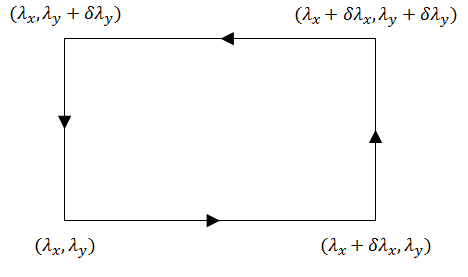
\includegraphics[width=0.5\textwidth]{squarrows}
\end{figure}
\footnotesize
\begin{equation*}
\begin{split}
  \oint_{Q}{\mathbf{A}_{n}(\bm{\lambda})\cdot \delta\bm{\lambda}} = -\arg(\braket{n(\bm{\lambda})|n(\bm{\lambda} + \delta\lambda_x \hat{\mathbf{x}})}\braket{n(\bm{\lambda} + \delta\lambda_x \hat{\mathbf{x}})|n(\bm{\lambda} + \delta\lambda_x \hat{\mathbf{x}} + \delta\lambda_y \hat{\mathbf{y}})}\\ \braket{n(\bm{\lambda} + \delta\lambda_x \hat{\mathbf{x}} + \delta\lambda_y \hat{\mathbf{y}})|n(\bm{\lambda} + \delta\lambda_y \hat{\mathbf{y}})}\braket{n(\bm{\lambda} + \delta\lambda_y \hat{\mathbf{y}})|n(\bm{\lambda})})
\end{split}
\end{equation*}
\begin{align*}
\oint_{Q}{\mathbf{A}_{n}(\bm{\lambda})\cdot \delta\bm{\lambda}} &= \int_{Q}{\mathbf{B}_{n}(\bm{\lambda})\cdot d\mathbf{S}_{\bm{\lambda}}}\\
  &= \mathbf{B}_{n}(\bm{\lambda}) \delta\lambda_x\delta\lambda_y 
\end{align*}
\normalsize
\end{frame}

\begin{frame}{Bargmann invariants}
\begin{equation*}
\oint_{Q}{\mathbf{A}_{n}(\bm{\lambda})\cdot \delta\bm{\lambda}} = \mathbf{B}_{n}(\bm{\lambda}) \delta\lambda_x\delta\lambda_y 
\end{equation*}
\begin{theorem}
\footnotesize
\begin{equation*}
\begin{split}
 \mathbf{B}_{n}(\bm{\lambda}) \delta\lambda_x\delta\lambda_y = -\arg(\braket{n(\bm{\lambda})|n(\bm{\lambda} + \delta\lambda_x \hat{\mathbf{x}})}\braket{n(\bm{\lambda} + \delta\lambda_x \hat{\mathbf{x}})|n(\bm{\lambda} + \delta\lambda_x \hat{\mathbf{x}} + \delta\lambda_y \hat{\mathbf{y}})}\\ \braket{n(\bm{\lambda} + \delta\lambda_x \hat{\mathbf{x}} + \delta\lambda_y \hat{\mathbf{y}})|n(\bm{\lambda} + \delta\lambda_y \hat{\mathbf{y}})}\braket{n(\bm{\lambda} + \delta\lambda_y \hat{\mathbf{y}})|n(\bm{\lambda})})
\end{split}
\end{equation*}
\end{theorem}
\normalsize
Surface integral of Berry Curvature can be converted into sum of 4-point Bargmann invariant at each point.
\end{frame}
\subsection{Chern numbers}
\begin{frame}{Chern numbers}{Topological Invariant}
\begin{theorem}[Gauss-Bonnet]
The surface integral of Gaussian curvature over a 2-dimensional closed Riemannian manifold is equal to $2\pi\chi$, where $\chi$ is the Euler characteristic of the manifold.
\end{theorem}
\begin{itemize}
 \item Euler characteristic of any manifold is an integer.
 \item Two homotopic surfaces have the same Euler characteristic.
 \item Intuitively, they are related to number of holes in the surface.
\end{itemize}

\alert{Berry curvature behaves like Gaussian curvature}. This topological invariant is also called the \alert{first Chern number}.
\end{frame}

\subsection{TKNN invariant}
\begin{frame}{TKNN invariant}{Particles on a Lattice}
On a rectangular 2D lattice, translation of the form $\mathbf{r} \rightarrow \mathbf{r}+\mathbf{R}$ where $\mathbf{R} = ma \;\hat{\mathbf{x}} + nb \;\hat{\mathbf{y}}\;\ni m,n\in\mathbb{Z}$,
does not affect the Hamiltonian.

From \alert{Bloch's theorem} the wavefunctions are of the form
\begin{equation}
 \ket{\psi_{\mathbf{k}}(\mathbf{r})} = e^{i\mathbf{k}\cdot\mathbf{r}} \ket{u_{\mathbf{k}}(\mathbf{r})}
\end{equation} such that $\ket{u_{\mathbf{k}}(\mathbf{r}+\mathbf{R})} = \ket{u_{\mathbf{k}}(\mathbf{r})}$.

$\mathbf{k}$ is the crystal momentum confined to limits of the Brillouin zone
\begin{equation*}
 \frac{-\pi}{a} \leq k_{x} \leq \frac{\pi}{a}\text{ and }\frac{-\pi}{b} \leq k_{y} \leq \frac{\pi}{b}
\end{equation*}

Each band in the spectrum is parameterized by $\mathbf{k}$ on a torus $\mathbf{T}^2$.
\end{frame}
\begin{frame}{TKNN invariant}{Particles on a Lattice}
\small The Brillouin zone torus is a closed 2D parameter space.
Berry connection on this parameter space is
\begin{equation}
 A_{x}^{\alpha}(\mathbf{k}) = i\braket{u_{\mathbf{k}}^{\alpha}|\frac{\partial}{\partial k_{x}}|u_{\mathbf{k}}^{\alpha}} \quad A_{y}^{\alpha}(\mathbf{k}) = i\braket{u_{\mathbf{k}}^{\alpha}|\frac{\partial}{\partial k_{y}}|u_{\mathbf{k}}^{\alpha}}
\end{equation}
Berry curvature 
\begin{equation}
 B_{z}^{\alpha} = \frac{\partial A_{x}^{\alpha}}{\partial k_{y}} - \frac{\partial A_{y}^{\alpha}}{\partial k_{x}}
\end{equation} where $\alpha$ is the band index.

Integral of Berry curvature over $\mathbf{T}^2$ is 
\begin{equation}
 \int_{\mathbf{T}^2}d^2k \;B_{z}^{\alpha} = 2\pi C_{\alpha}
\end{equation}
\alert{$C_{\alpha}$ is an integer - a Chern number}, also called the \alert{TKNN invariant}.\normalsize
\end{frame}

\section{Quantum Hall Effect}
\subsection{Phenomenon}
\begin{frame}{Quantum Hall Effect}{Phenomenon}
Experiments by von Klitzing et al., showed that Hall conductivity exists on quantized plateaus as magnetic field is increased.
\begin{figure}[h]
 \centering
 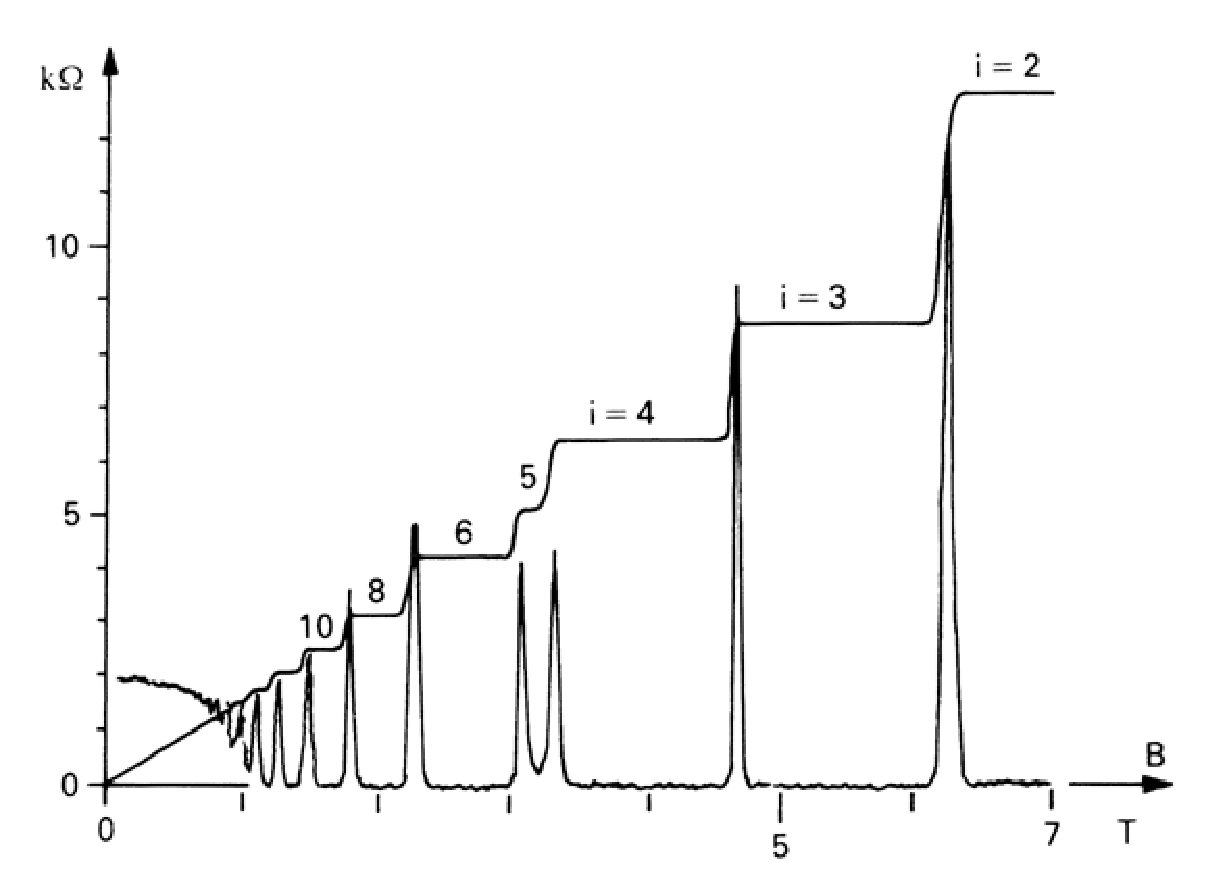
\includegraphics[width=0.5\textwidth]{ihall}
\end{figure}
\end{frame}
\begin{frame}{Quantum Hall Effect}{Phenomenon}
\begin{itemize}
 \item Conductivity on these plateaus take the value $\sigma_{x,y} = \frac{e^2}{2\pi\hbar}v \quad v \in \mathbb{Z}$.
 \item The centre of each plateau occurs when the magnetic field $B = \frac{2\pi\hbar n}{ve}$ where $n$ is the electron density. This is the magnetic field at which
 $v$ Landau levels are filled.
 \item Despite the presence of disorders, the observations do not change.
\end{itemize}
 Explanation in terms of filled Landau levels, Edge modes and Spectral Flow was given by \emph{Laughlin}.
 
 Thouless et al., explained Integer Quantum Hall effect using the \alert{Kubo formula}.
\end{frame}

\subsection{Kubo formula}
\begin{frame}{Kubo formula for Electrical Conductivity}{Linear Response Theory}
 Kubo formula is a result of linear response theory. The linear correlation between applied electric field (stimulus) and the resulting current density (response) is given by
 the Kubo formula for Electrical Conductivity.\footnotesize
 \begin{gather}
 J_{x} = \sigma_{xy} E_{y} \\
 \sigma_{xy} = i\hbar \sum_{\alpha,\beta | E_{\alpha}<E_{F}<E_{\beta}}\int_{\mathbf{T}^2}\frac{d^2 k}{(2\pi)^2} \frac{\braket{u_k^\alpha |J_{y}|u_k^\beta}\braket{u_k^\beta |J_{x}|u_k^\alpha} - \braket{u_k^\alpha |J_{x}|u_k^\beta}\braket{u_k^\beta |J_{y}|u_k^\alpha}}{(E_{\beta}(\mathbf{k})-E_{\alpha}(\mathbf{k}))^2}
\end{gather}\normalsize
$E_{F}$ is the Fermi energy.
\end{frame}

\begin{frame}{Kubo formula for Electrical Conductivity}{TKNN invariant}
 Using the definition of current density in terms of group velocity of wavepackets
 \begin{equation*}
  \tilde{H} = e^{-i\mathbf{k}\cdot\mathbf{x}}He^{i\mathbf{k}\cdot\mathbf{x}}\qquad \mathbf{J} = \frac{e}{\hbar}\frac{\partial \tilde{H}}{\partial \mathbf{k}}
 \end{equation*} the Kubo formula can be recast as
 \begin{equation}
  \sigma_{xy} = \frac{ie^2}{\hbar}\sum_{\alpha}\int_{\mathbf{T}^2}\frac{d^2k}{(2\pi)^2}\; \braket{\partial_{y}u_{\mathbf{k}}^{\alpha}|\partial_{x}u_{\mathbf{k}}^{\alpha}} - \braket{\partial_{x}u_{\mathbf{k}}^{\alpha}|\partial_{y}u_{\mathbf{k}}^{\alpha}}
 \end{equation} where $\partial_{x} = \frac{\partial}{\partial k_{x}}$ and $\partial_{y} = \frac{\partial}{\partial k_{y}}$.

 Amazingly, the integral is exactly same as the one for TKNN invariant.
\begin{equation}
 \sigma_{xy} = -\frac{e^2}{2\pi\hbar}\sum_{\alpha}C_{\alpha}
\end{equation}
\end{frame}

\begin{frame}{TKNN result}
 \begin{theorem}
 Hall Conductivity is a topological invariant.
\end{theorem}

The Hall conductivity cannot change continuously. It takes discrete jumps. Any deformation that does not change the underlying topology of the vector line bundle does not affect
Hall Conductivity.

\alert{Caution} : This result is only valid at absolute zero $T = 0 K$. We have no way to extend this result to time-varying Hamiltonians as of now.
\end{frame}

\section{Floquet theory}
\subsection{Statement}
\begin{frame}{Floquet Theory}{Statement}
 \begin{theorem}[Floquet Theory]\footnotesize
 Solutions to time-dependent Schrodinger equation 
 \begin{equation*}
  i\hbar\frac{\partial}{\partial t}\ket{\psi(t)} = \hat{H}(t)\ket{\psi(t)}
 \end{equation*} where $\hat{H}(t)$ is periodic $\quad \forall t \quad \hat{H}(t+T) = \hat{H}(t)$
 are of the form
 \begin{equation*}
  \ket{\psi_{\alpha}(t)} = e^{-i\epsilon_{\alpha}t} \ket{\phi_{\alpha}(t)}
 \end{equation*}
 \end{theorem}
 \begin{itemize}  
  \item There are $n = dim(H)$ independent solutions indexed by $\alpha$.
  \item $\ket{\psi_{\alpha}(t)}$ -- \emph{Floquet states}.
  \item $\ket{\phi_{\alpha}(t)}$ -- \emph{Floquet modes}.
  \item $\epsilon_{\alpha}$ -- \emph{Quasienergies}.
 \end{itemize}\normalsize
\end{frame}

\begin{frame}{Floquet Theory}{Corollaries}
\small
\begin{align*}
  \ket{\psi_{\alpha}(t+T)} &= \mathit{e}^{-i \epsilon_{\alpha} (t+T)} \ket{\phi_{\alpha}(t+T)} \\
  &= \mathit{e}^{-i \epsilon_{\alpha} T} \mathit{e}^{-i \epsilon_{\alpha} t} \ket{\phi_{\alpha}(t)} \\  
  &= \mathit{e}^{-i \epsilon_{\alpha} T} \ket{\psi_{\alpha}(t)}
\end{align*}
\begin{itemize}
 \item $\epsilon_{\alpha}$ is real. (Normalization)
 \item If $\hat{U}(t_2, t_1)$ is the time evolution operator, then 
 \begin{equation*}
  \hat{U}(t + T, t)\ket{\psi_{\alpha}(t)} = \mathit{e}^{-i \epsilon_{\alpha} T} \ket{\psi_{\alpha}(t)}
 \end{equation*}
 Floquet states at any time $t$ form a complete orthonormal basis.
 \item $\epsilon_\alpha$ may be replaced by $\epsilon_{\alpha n}=\epsilon_\alpha + n\omega$ without affecting the above equations.
 Restrict $\epsilon_\alpha \in \left[\frac{-\omega}{2}, \frac{\omega}{2}\right)$, called the \emph{Floquet Brillouin zone}.
\end{itemize}\normalsize
\end{frame}
\begin{frame}{Floquet Theory}{Corollaries}
\small
\begin{align*}
  \hat{U}(t_2, t_1) &= \sum_{\alpha_2}{\ket{\psi_{\alpha_2}(t_2)}\bra{\psi_{\alpha_2}(t_2)}}\hat{U}(t_2, t_1)\sum_{\alpha_1}{\ket{\psi_{\alpha_1}(t_1)}\bra{\psi_{\alpha_1}(t_1)}} \nonumber \\
  &= \sum_{\alpha_1, \alpha_2}{\ket{\psi_{\alpha_2}(t_2)}\braket{\psi_{\alpha_2}(t_2)|\psi_{\alpha_1}(t_2)}\bra{\psi_{\alpha_1}(t_1)}} \nonumber \\
  &= \sum_{\alpha}{e^{-i\epsilon_\alpha (t_2 - t_1)} \ket{\phi_\alpha (t_2)}\bra{\phi_\alpha (t_1)}}
\end{align*}
\normalsize
We can therefore express any $\ket{\psi(t)}$ as
\begin{equation*}
  \ket{\psi(t)} = \sum_{\alpha}{\braket{\phi_\alpha (t_0) | \psi(t_0)} e^{-i\epsilon_\alpha (t - t_0)} \ket{\phi_\alpha (t)}} 
\end{equation*} i.e., the contribution of each floquet mode remains constant as the state evolves in time.
\end{frame}

\begin{frame}{Floquet Theory}{Macromotion and Micromotion}\small
The time-evolution operator over one-time period $\hat{U}(t_0 + T, t_0)$ is the \emph{Macromotion/Strobosscopic} operator.
We designate $\hat{H}_{t_0}^{F}$ from $\exp\left(-iT\hat{H}_{t_0}^{F}\right) = \hat{U}(t_0 + T, t_0)$ as the \emph{Floquet Hamiltonian}.
Floquet Hamiltonian satisfies
\begin{equation}
 \hat{H}_{t_0}^{F}\ket{\phi_\alpha (t_0)} = \epsilon_\alpha \ket{\phi_\alpha (t_0)}
\end{equation}

The \emph{Micromotion} operator is
\begin{gather}
  \ket{\phi_\alpha (t_2)} = \hat{U}_{F}(t_2, t_1)\ket{\phi_\alpha (t_1)}\\
  \hat{U}_{F}(t_2, t_1) = \sum_{\alpha}{\ket{\phi_\alpha (t_2)}\bra{\phi_\alpha (t_1)}}
\end{gather} which describes the time evolution of periodic floquet modes.
\normalsize \end{frame}

\begin{frame}{Floquet Theory}
\begin{itemize}
 \item Floquet Hamiltonian is time-independent but parameterized by initial time $t_0$. It holds all the information regarding the system.
 \item By diagonalizing the Floquet Hamiltonian, the Quasienergies and the Floquet modes can be determined.
 \item However, we have not yet described a procedure to calculate the Floquet Hamiltonian from the original Hamiltonian.
 \item A myriad of approximation schemes to obtain the Floquet Hamiltonian have been designed. We discuss two such methods.
\end{itemize}
\end{frame}

\subsection{Perturbation techniques}
\begin{frame}{Floquet Theory}{Effective Hamiltonian}
 The Floquet modes satisfy the following eigenvalue equation
  \begin{equation*}
    \left[\hat{H} - i\frac{\partial}{\partial t}\right]\ket{\phi_\alpha} = \epsilon_\alpha\ket{\phi_\alpha}
  \end{equation*} This is an alternative definition to Floquet Hamiltonian. We call this the \emph{Quasienergy operator}.
  
  \begin{equation}
   \hat{Q} = \left[\hat{H} - i\frac{\partial}{\partial t}\right]
  \end{equation}
  
  Floquet Hamiltonian is parameterized by initial time. Define a static Hamiltonian without any initial time parameter without losing the
  physical interpretation of macromotion.
\end{frame}

\begin{frame}{Effective Hamiltonian}
 Let $\hat{U}_{F}(t)$ be a unitary transformation, such that
 \begin{equation}
  \hat{H}_{F} = \hat{U}_{F}(t)\hat{Q}(t)\hat{U}_{F}^{\dagger}(t)
 \end{equation} is time-independent.
 
 Under this transformation
 \begin{itemize}
  \item Macromotion operator $\hat{H}_{F}$ is independent of initial time.
  \item Floquet modes $\ket{\phi_\alpha^{F}} = \hat{U}_{F}(t)\ket{\phi_\alpha (t)}$ are time-independent.
  \item Micromotion operator $\hat{U}_{F}(t_2, t_1) = \hat{U}_{F}^{\dagger}(t_2)\hat{U}_{F}(t_1)$.
  \item Time-evolution operator $\hat{U}(t_2, t_1) = \hat{U}_{F}^{\dagger}(t_2)e^{-i\hat{H}_{F}(t_2 - t_1)}\hat{U}_{F}(t_1)$
 \end{itemize}
\end{frame}

\begin{frame}{Effective Hamiltonian}
\begin{enumerate}
 \item Enforce periodicity on $\hat{U}_{F}(t) = \hat{U}_{F}(t+T)$.
 \item Rewrite $\hat{U}_{F}(t)$ as $e^{i\hat{K}(t)}$ where $\hat{K}(t)$ is called the \emph{Kick operator}.
 \item Expand Hamiltonian in Fourier series $\hat{H}(t) = \hat{H}_{(0)} + \sum_{j=1}^{\infty}{\hat{H}_{(j)} e^{ij\omega t} + \hat{H}_{(-j)} e^{-ij\omega t}}$
 \item Perturbation ansatz :  $\hat{H}_{F}(t) = \sum_{j=0}^{\infty}{\frac{1}{\omega^j}\hat{H}_{F}^{(j)}}$.
 \item Perturbation ansatz : $\hat{K}(t) = \sum_{j=0}^{\infty}{\frac{1}{\omega^j}\hat{K}^{(j)}}$.
\end{enumerate}
In the high-frequency limit, contributions from higher order terms is negligible.
With this ansatz, expressions for $\hat{H}_{F}$ and $\hat{K}_{F}$ can be obtained.

$\hat{H}_{F}$ is called the \alert{Effective Hamiltonian}.
\end{frame}

\begin{frame}{Brillouin-Wigner Perturbation}{Concept}
Let us introduce some terminology \small
\begin{itemize}
 \item \textbf{Reference states} : $\mathbf{R}$ is a complete set of orthonormal states of the Hilbert space.
 \item \textbf{Model State} : One chosen state $\ket{\phi_0}$ from $\mathbf{R}$.
 \item \textbf{Model Space} : One dimensional complex vector space with Model State as the basis.
 \item \textbf{Orthogonal Space} : Hilbert Space $-$ Model Space
 \item \textbf{Projection Operator} : Projects to Model space $P = \ket{\phi_0}\bra{\phi_0}$. $P$ transports a vector from Hilbert space to Model space. $\ket{\phi} = P\ket{\psi}$ 
 \item \textbf{Orthogonal Projection Operator} : $Q = 1 - P$.
 \item \textbf{Wave Operator} : Reconstructs Hilbert Space wavefunction from Model space wavefunction. $\ket{\psi} = \Omega\ket{\phi}$ 
\end{itemize} \normalsize
\end{frame}

\begin{frame}{Brillouin-Wigner Perturbation}{Concept}
 We intend to solve
 \begin{equation*}
  \hat{H}\ket{\psi} = E\ket{\psi}
 \end{equation*}

 If $\ket{\phi} = P\ket{\psi}$, then
 \begin{equation}
  \hat{H}_{eff}\ket{\phi} = E\ket{\phi}
 \end{equation} where
 \begin{equation}
  \hat{H}_{eff} = P\hat{H}\Omega P
 \end{equation}
 
 Diagonalizing the Effective Hamiltonian $\hat{H}_{eff}$ in turn solves the original eigenvalue problem.
 
 $\Omega$ is obtained as
 \begin{equation}
    \Omega = \left(1-\frac{Q\hat{H}}{E}\right)^{-1}P
 \end{equation}
\end{frame}

\begin{frame}{Brillouin-Wigner Perturbation}{Floquet Hamiltonian}
 $\hat{H}$, $\ket{\phi}$ are periodic in time. They are expanded in Fourier series.
 
 Let
 \begin{gather}
  \mathcal{H}_{m,n} = \frac{1}{T}\int_{0}^{T}e^{i(m-n)t}\hat{H}(t)\,dt \\
  \mathcal{M}_{m,n} = m\delta_{m,n}\\
  \ket{\phi_{\alpha}^{m}} = \frac{1}{T}\int_{0}^{T}e^{imt}\ket{\phi_{\alpha}}\,dt
 \end{gather}
 
 Then
 \begin{equation}
  (\mathcal{H} - \mathcal{M}\omega)\ket{\phi_{\alpha}} = \epsilon_{\alpha}\ket{\phi_{\alpha}}
 \end{equation}
 Apply Brillouin-Wigner Perturbation theory to solve above equation.
\end{frame}
\begin{frame}{Brillouin-Wigner Perturbation}{Effective Hamiltonian}
\begin{itemize}
 \item Choose Fourier modes as the Reference states.
 \item Project to static fourier mode. $\mathcal{P} = \delta_{m,n}\delta_{m,0}$
 \item Obtain Wave operator $\Omega$ and $\hat{H}_{eff}$.
 \item Further simplified by defining $E$ independent $\Omega$ called $\Omega_{BW}$.
Obtain $\hat{H}_{BW} = \mathcal{P}\mathcal{H}\Omega_{BW}\mathcal{P}$.
$\hat{H}_{BW}$ is time-independent because we are in Fourier basis.
\item $\Omega_{BW}$ is expanded in a $1/\omega$ series.
\end{itemize}

\tiny \alert{Details are omitted for brevity.} \normalsize
\end{frame}

\section{Aubry-Andr\'{e}-Harper Model}
\subsection{Introduction}
\begin{frame}{Aubry-Andr\'{e}-Harper Model}{Problem Description}
 \begin{itemize}
  \item Motion of electrons (spinless, non-relativistic) in a periodic 2-dimensional rectangular lattice subject to a constant magnetic field perpendicular to the plane of the lattice.
  \item Landau-level problem on a lattice.
 \end{itemize}
Hamiltonian in the presence of magnetic field is obtained by replacing $\hat{\mathbf{p}}$ by $\hat{\mathbf{p}} - e\mathbf{A}$.
\begin{equation}
 \hat{H}(x, y) = \frac{1}{2m}(\hat{\mathbf{p}} - e\mathbf{A})^2 + \hat{V}(x,y)
\end{equation}
\end{frame}

\begin{frame}{Aubry-Andr\'{e}-Harper Model}{Bloch's theorem in the presence of Magnetic field}
 \begin{itemize}
  \item Uniform Magnetic field $\mathbf{B} = B\hat{\mathbf{z}}$
  \item Magnetic Vector Potential in Landau gauge $\mathbf{A} = Bx\hat{\mathbf{y}}$
 \end{itemize}
Hamiltonian has no translational invariance $\mathbf{A}(\mathbf{r}) \neq \mathbf{A}(\mathbf{r} + \mathbf{R})$.
The Translation Operators do not commute with the Hamiltonian rendering Bloch's theory useless.
\end{frame}

\begin{frame}{Aubry-Andr\'{e}-Harper Model}{Bloch's theorem in the presence of Magnetic field}
 \small For uniform magnetic field
 \begin{equation*}
 \mathbf{A}(\mathbf{r} + \mathbf{R}) = \mathbf{A}(\mathbf{r}) + \bm{\nabla}\mathcal{G}(\mathbf{r}, \mathbf{R})
\end{equation*}
Therefore, the operation of translation operator on the Hamiltonian is equivalent to a gauge transformation
\begin{gather*}
 \hat{T}_{\mathbf{R}}\left(\frac{1}{2m}(\hat{\mathbf{p}} - e\mathbf{A}(\mathbf{r}))^2\right) = \left(\frac{1}{2m}(\hat{\mathbf{p}} - e\mathbf{A}(\mathbf{r}) - e\bm{\nabla}\mathcal{G}(\mathbf{r}, \mathbf{R}))^2\right)\hat{T}_{\mathbf{R}} \\
 \label{chap_6:magneticgaugetransform}\left(\frac{1}{2m}(\hat{\mathbf{p}} - e\mathbf{A}(\mathbf{r}) - e\bm{\nabla}\mathcal{G}(\mathbf{r}, \mathbf{R}))^2\right) = e^{\frac{ie}{\hbar}\mathcal{G}(\mathbf{r}, \mathbf{R})}\left(\frac{1}{2m}(\hat{\mathbf{p}} - e\mathbf{A}(\mathbf{r}))^2\right)e^{\frac{-ie}{\hbar}\mathcal{G}(\mathbf{r}, \mathbf{R})}
\end{gather*}
\alert{Magnetic translation operators}
\begin{equation*}
 \hat{\mathcal{T}}_{\mathbf{R}} = e^{\frac{-ie}{\hbar}\mathcal{G}(\mathbf{r}, \mathbf{R})}\hat{T}_{\mathbf{R}}
\end{equation*} commutes with $\hat{H}$.
\normalsize
\end{frame}

\begin{frame}{Aubry-Andr\'{e}-Harper Model}{Bloch's theorem in the presence of Magnetic field}
 For Magnetic Translation operators to form a group
 \begin{equation*}
 \hat{\mathcal{T}}_{\mathbf{R}}\hat{\mathcal{T}}_{\mathbf{R}'} = e^{\frac{-ie}{\hbar}BR_{x}'R_{y}}\hat{\mathcal{T}}_{\mathbf{R} + \mathbf{R}'}
 \end{equation*}
 we need
 \begin{equation*}
 \alpha = \frac{e}{h}Bd^2 = \frac{p}{q} \text{ such that } p,q \in \mathcal{Z}^{+} \text{ and } gcd(p, q) = 1
\end{equation*} and define \emph{Magnetic Translation vectors}
\begin{equation*}
 \mathcal{R} = qmd \hat{\mathbf{x}} + nd \hat{\mathbf{y}} \text{ such that } m,n \in \mathcal{Z}
\end{equation*} then, a subset of magnetic translation operators, that translate by units of magnetic unit cell form a group
\begin{equation*}
 \hat{\mathcal{T}}_{\mathcal{R}}\hat{\mathcal{T}}_{\mathcal{R}'} = e^{-i2\pi\frac{e}{h}Bm_{1}n_{2}qd^2}\hat{\mathcal{T}}_{\mathcal{R} + \mathcal{R}'} = e^{-i2\pi p m_{1}n_{2}}\hat{\mathcal{T}}_{\mathcal{R} + \mathcal{R}'} = \hat{\mathcal{T}}_{\mathcal{R} + \mathcal{R}'}
\end{equation*}
\end{frame}

\begin{frame}{Aubry-Andr\'{e}-Harper Model}{Bloch's theorem in the presence of Magnetic field}\small
 This redefinition of Translation vectors also defines the \alert{Magnetic Brillouin Zone}
\begin{equation*}
 k_{x} \in \left(-\frac{\pi}{q},\frac{\pi}{q}\right) \text{ and } k_{y} \in (-\pi,\pi)
\end{equation*}
Now we can write the Bloch's theorem like equation
\begin{equation*}
 \hat{\mathcal{T}}_{\mathcal{R}}\ket{\psi_{\mathbf{k}}(\mathbf{r})} = e^{i\mathbf{k}\cdot\mathcal{R}}\ket{\psi_{\mathbf{k}}(\mathbf{r})}
\end{equation*}
\begin{equation*}
 \ket{\psi_{\mathbf{k}}(\mathbf{r})} = e^{i\mathbf{k}\cdot\mathbf{r}}\ket{u_{\mathbf{k}}(\mathbf{r})}
\end{equation*}
However, $\ket{u_{\mathbf{k}}(\mathbf{r}+\mathcal{R})} \neq \ket{u_{\mathbf{k}}(\mathbf{r})}$. Rather,
\begin{equation*}
 \ket{u_{\mathbf{k}}(\mathbf{r} + \mathcal{R})} = e^{-i2\pi\frac{e}{h}Bqmdy}\ket{u_{\mathbf{k}}(\mathbf{r})}
\end{equation*} This is called the \emph{Generalized bloch condition}. \normalsize
\end{frame}

\subsection{Tight-Binding Hamiltonian}
\begin{frame}{Tight-Binding Model}
 The wavefunction is expanded as a linear combination of a set of localized states - Wannier/single atom states.
 \begin{equation*}
 \ket{\psi(\mathbf{r})} = \sum_{\mathbf{R}}{a_{\mathbf{R}} \ket{\phi_{\mathbf{R}}(\mathbf{r})}}
\end{equation*} where $\braket{\phi_{\mathbf{R}'}|\phi_{\mathbf{R}}} = \delta_{m'm}\delta_{n'n}$.

Generic Tight-Binding model is written as
\begin{equation}
 W_{1,0}(a_{m+1, n} + a_{m-1, n}) + W_{0, 1}(a_{m, n+1} + a_{m, n-1}) = Ea_{m, n}
\end{equation}
In matrix form
\begin{equation*}
\hat{H}_{0} = \sum_{m,n} W_{1,0}\ket{m+1, n}\bra{m, n} + W_{0,1}\ket{m, n+1}\bra{m, n} + h.c.
\end{equation*}
\end{frame}

\begin{frame}{Tight-Binding Model}{Peirels Substitution}\small
In the presence of magnetic field, we expand as
\begin{equation*}
 \ket{\psi(\mathbf{r})} = \sum_{\mathbf{R}}{a_{\mathbf{R}} e^{2\pi \frac{ie}{h}\int_{\mathbf{R}}^{\mathbf{r}}{\mathbf{A}\cdot d\mathbf{r}'}}\ket{\phi_{\mathbf{R}}(\mathbf{r})}}
\end{equation*} This leads to the tight-binding Hamiltonian
\begin{equation*}
 \hat{H} = \sum_{m, n} W_{1,0}\ket{m+1, n}\bra{m, n} + W_{0,1}e^{2\pi i \alpha m}\ket{m, n+1}\bra{m, n} + h.c.
\end{equation*} where $\alpha = \frac{eBd^2}{h}$ is the magnetic flux through an unit cell.
Coefficients in the above equation, involve only $m$ and do not depend on $n$.
Plane-wave behaviour in y-direction $a_{mn} = e^{in\theta}a_m$.
\begin{equation}
 a_{m+1} + a_{m-1} + \lambda \cos(2\pi m \alpha + \theta)a_{m} = Ea_{m}
\end{equation}
This is known as the \alert{Harper's equation} for $\lambda=2$.\normalsize
\end{frame}

\subsection{Spectrum}
\begin{frame}{Harper Model}{Spectrum}
\begin{figure}[h]
 \centering
 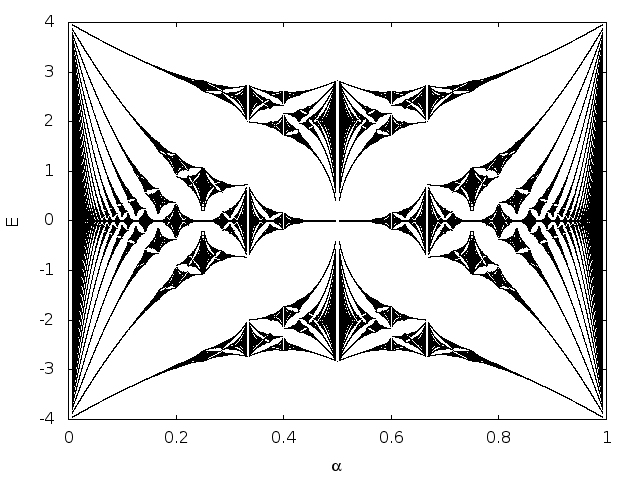
\includegraphics[width=0.7\textwidth]{butterfly}
\end{figure} 
\end{frame}

\begin{frame}{Harper Model}{Spectrum}
\begin{columns}
 \begin{column}{0.35\textwidth}
  \begin{figure}[h]
    \centering
    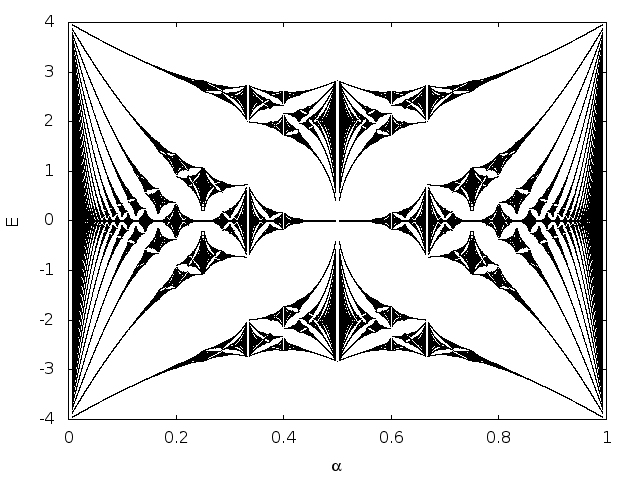
\includegraphics[width=\textwidth]{butterfly}
  \end{figure} 
 \end{column}
 \begin{column}{0.65\textwidth}
  \begin{itemize}\small
  \item $\alpha$ and $N+\alpha$ produce the same spectrum. $\alpha$ may be restricted to $[0,1]$ for this reason.
  \item The energy eigenvalues are symmteric with respect to zero. i.e., if $\epsilon \in spectrum(\alpha)$, then $-\epsilon \in spectrum(\alpha)$.
  \item $|\epsilon| \leq 4$.
  \item The energy eigenvalues of irrational $\alpha$ is homeomorphic to a cantor set.
  \item The graph has a recursive structure.
 \end{itemize}\normalsize
 \end{column}
\end{columns}
\end{frame}

\subsection{Metal-Insulator Phase Transition}
\begin{frame}{Localization/Delocalization}{Inverse Participation Ratio}
 \alert{IPR} is defined as
 \begin{equation}
 IPR = \frac{\sum_{n=1}^{L} |a_{n}|^4} {(\sum_{n=1}^{L} |a_{n}|^2)^2}
\end{equation}
$a_n$'s are the coefficients of the eigenstates in some basis.

IPR lies in the range $1$ to $1/L$, where $1$ indicates a perfectly localized state and $1/L$ indicates a perfectly delocalized state.
\end{frame}

\begin{frame}{Aubry-Andr\'e-Harper Model}{Localization/Delocalization}
 \begin{figure}[h]
\caption{\tiny The metal-to-insulator transition of the
AAH Hamiltonian for the system’s ground state. Plot (a) shows the
IPR versus $V_0$ or $\lambda$ in real space for L = 144, 1597 and 10 946 (top to
bottom) with $\alpha_0 = (\sqrt(5)-1)/2$ (inverse of golden ratio). The inset shows the variation of $D_2$ with $V_0$ which also
exhibits a transition. Plot (b) exhibits the mirror behavior in the dual
space\normalsize}
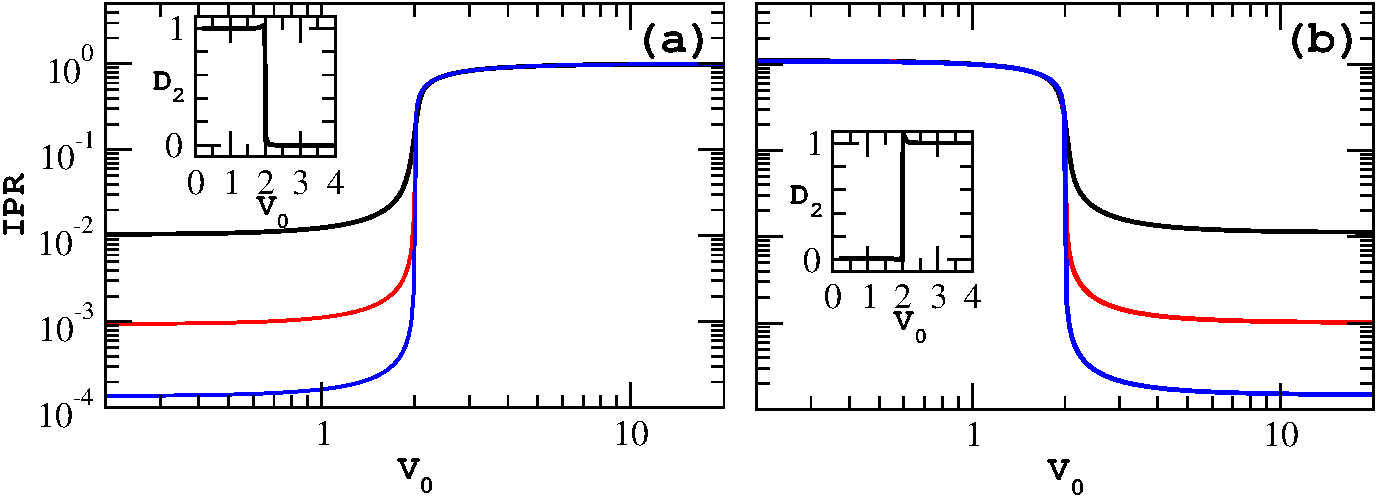
\includegraphics[width=0.75\textwidth]{AA-IPR-D2-Vs-V1byV2}
\centering
\end{figure}
\end{frame}

\begin{frame}{Aubry-Andr\'e-Harper Model}{Localization/Delocalization}
 \begin{columns}
  \begin{column}{0.5\textwidth}
    \begin{figure}[h]
      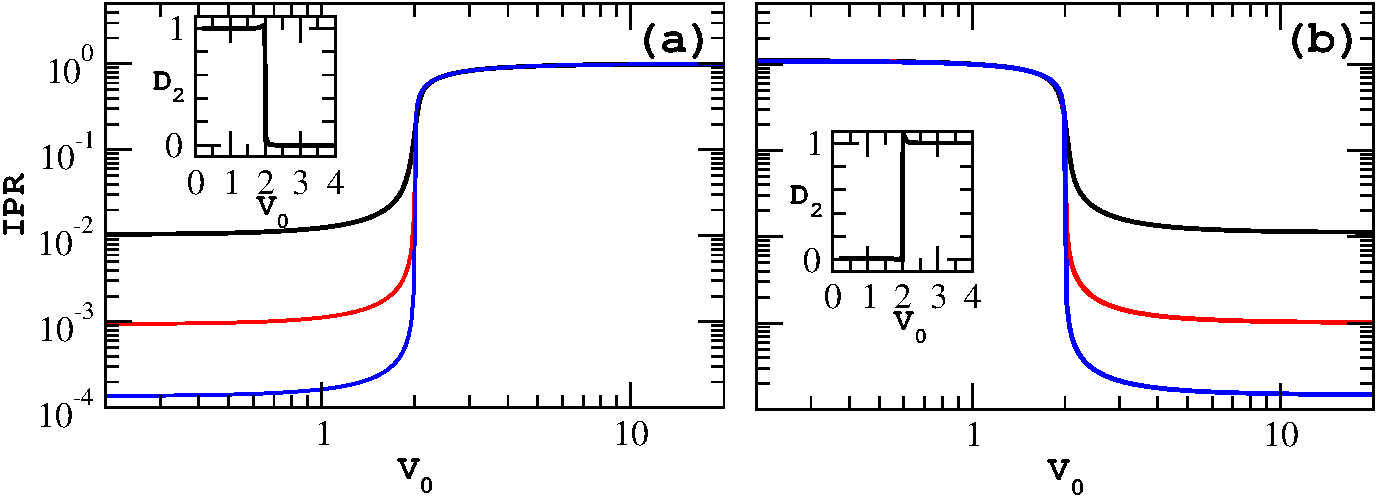
\includegraphics[width=\textwidth]{AA-IPR-D2-Vs-V1byV2}
      \centering
      \end{figure}
  \end{column}
  \begin{column}{0.5\textwidth}
   AAH model has a duality transformation
    \begin{equation*}
    \ket{m} = \frac{1}{\sqrt{L}}\sum_{n}e^{-i2\pi\alpha_0 m n} \ket{n}
    \end{equation*}
    Wavefunctions localized in real space are delocalized in the dual space and vice versa.
  \end{column}
 \end{columns}
\end{frame}

\subsection{Chern numbers}
\begin{frame}{Aubry-Andr\'e-Harper Model}{Hall Conductivity}
First model for which relationship between Hall Conductivity and Chern numbers was established.
Tight-binding Hamiltonian in Momentum space is obtained by Fourier transform
\begin{align}
 \ket{m, n} &= \int_{-\pi}^{\pi}\int_{-\pi}^{\pi}\frac{dk_{x}}{2\pi}\frac{dk_{y}}{2\pi}e^{ik_xm+ik_yn}\ket{k_x, k_y} \\
 \bra{m, n} &= \int_{-\pi}^{\pi}\int_{-\pi}^{\pi}\frac{dk_{x}}{2\pi}\frac{dk_{y}}{2\pi}e^{-ik_xm-ik_yn}\bra{k_x, k_y}
\end{align} \small where $-\pi \leq k_x, k_y < \pi$ and $\ket{k_x + 2\pi a, k_y + 2\pi b} = \ket{k_x, k_y}$ where $a, b \in \mathbb{Z}$. \normalsize
\end{frame}

\begin{frame}{Aubry-Andr\'e-Harper Model}{Hall Conductivity}
 We obtain \footnotesize
  \begin{equation*}
    H_{ij} = 2W_{1,0} \cos(k_y + 2\pi\alpha m) \delta_{ij} + W_{0,1} (\delta_{i+1, j} + \delta_{i, j+1}) + W_{0,1}\delta_{i,q}\delta_{j,1} e^{ik_{x}^0 q} + W_{0,1}\delta_{i,1}\delta_{j,q} e^{-ik_{x}^0 q}
  \end{equation*} \normalsize
  
  It is a $q \times q$ matrix, each eigenvalue corresponding to one of the q-subbands.
  
  \begin{align*}
    \hat{H}(k_{x}^0, k_y) &= \hat{H}(k_{x}^0 + 2\pi/q, k_y) \\
    \hat{H}(k_{x}^0, k_y) &= \hat{H}(k_{x}^0, k_y+2\pi)
  \end{align*} The parametric dependence of $\hat{H}$ on $k_x^0 , k_y$ is described by a torus.
\end{frame}

\begin{frame}{Aubry-Andr\'e-Harper Model}{Chern numbers}
\begin{columns}
 \begin{column}{0.5\textwidth}
  \begin{figure}[h]
 \centering
 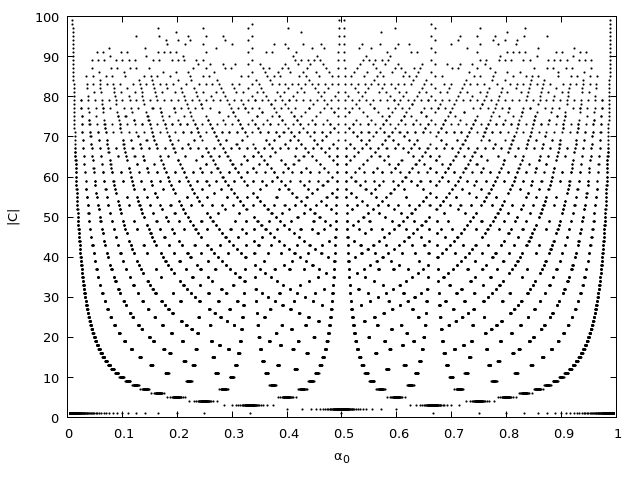
\includegraphics[width=\textwidth]{chern} 
\end{figure}
 \end{column}
 \begin{column}{0.5\textwidth}
   \begin{itemize}
  \item Chern numbers calculated on a Discretized Magnetic Brillouin zone.
  \item Sum of Four-point Bargmann Invariant for each point.
  \item Non-abelian Berry Curvature is required to tackle the degeneracy issues.
 \end{itemize}
 \end{column}
\end{columns}
\end{frame}

\section{Driven models}
\subsection{Oscillating Magnetic Field}

\begin{frame}{Driven Aubry-Andr\'e-Harper Model}{Oscillating Magnetic Field}
\begin{itemize}
 \item The magnetic field perpendicular to the 2D lattice plane is rapidly oscillating.
 \item As the magnetic field oscillates, what happens to the q-subband structure? 
 \item $q$ is an extremely discontinuous function of time and it cannot be ascribed a closed form expression.
 \item Time-independent effective Hamiltonian using Floquet theory!
\end{itemize}
\end{frame}

\begin{frame}{Driven Aubry-Andr\'e-Harper Model}{Effective Hamiltonian}
In Landau gauge, $\mathbf{A}(t) = Bx \cos(\omega t) \hat{\mathbf{y}}$.
Hamiltonian in tight-binding form \footnotesize
\begin{equation}
 \hat{H} = \sum_{n} \ket{n}\bra{n+1} + \ket{n}\bra{n-1} + V_{0}\cos(2\pi\alpha_{0}n\cos(\omega t) + \theta)\ket{n}\bra{n}
\end{equation}\normalsize

\small
 The static Effective Hamiltonian for this problem is calculated using the approach described earlier.
 \begin{itemize}
  \item In position space, the Effective Hamiltonian retains the tri-diagonal structure.
  \item The on-site term is a site-dependent oscillatory function because of appearance of $\mathcal{J}_{i}$ - Bessel functions.
  \item Upper and Lower diagonal terms are fixed at one.
  \item This model is not self-dual. The duality transformation described above does not retain the tri-diagonal structure.
 \end{itemize} \normalsize
\end{frame}

\begin{frame}{Driven Aubry-Andr\'e-Harper Model}{Metal-Insulator transition}
 \begin{figure}[h]
  \centering
  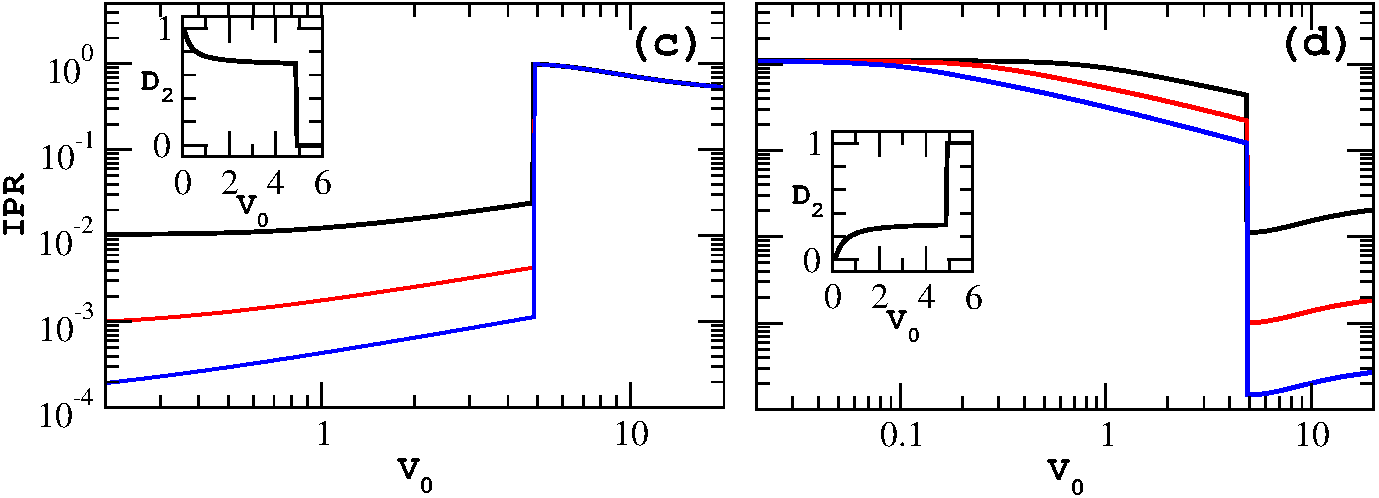
\includegraphics[width=0.85\textwidth]{FAA-Phase0-IPR-D2-Vs-V1byV2}  
  \end{figure}
\end{frame}

\begin{frame}{Driven Aubry-Andr\'e-Harper Model}{Energy-dependent Mobility edge}
\footnotesize Presence of energy-dependent mobility edge, an edge that splits the spectrum into two regions, one containing localized states and 
other containing delocalized states. This is a significant result as the mobility edge is atypical of 1-dimensional models. \normalsize
\begin{figure}[h]
\centering
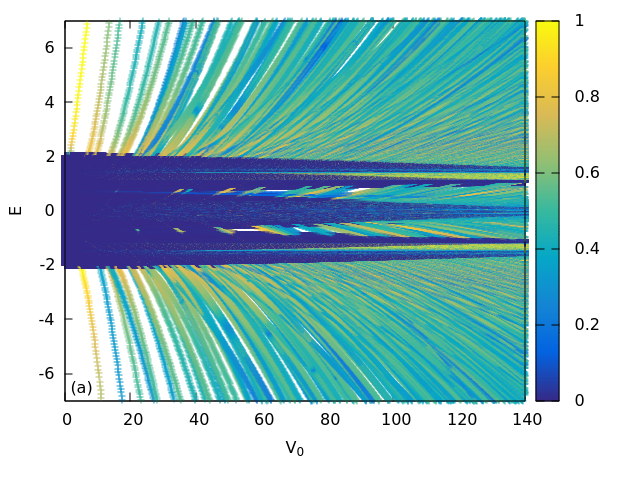
\includegraphics[width=0.50\textwidth]{evipr-4181-0.png}
\end{figure}
\end{frame}

\subsection{Linearly Polarized Light}
\begin{frame}{Driven Aubry-Andr\'e-Harper Model}{Linearly Polarized Electric Field}
\begin{itemize}
 \item Additional Linear Electric Field along one of the axes of the lattice.
 \item Magnetic Translation Operators change only by a constant phase factor.
 \item Magnetic Translation Group can still be constructed.
 \item q-subband structure is also unaffected.
 \item Using BW perturbation we perturbatively obtain the effective Hamiltonian.
\end{itemize}
\end{frame}

\begin{frame}{Driven Aubry-Andr\'e-Harper Model}{Linearly Polarized Electric Field}
 The magnetic vector potential corresponding to the system is\footnotesize
\begin{equation*}
 \mathbf{A}(t) = (Bx + A\cos(\omega t)) \hat{\mathbf{y}}
\end{equation*}\normalsize

The Hamiltonian in position space is
\begin{equation}
 a_{n+1} + a_{n-1} + 2\lambda\cos(2\pi(\alpha_0 + \alpha \cos{\omega t}) + \theta) a_{n} = E a_{n}
\end{equation} where $\alpha_0 = \frac{e}{h}Bd^2$ and $\alpha = \frac{e}{h}Ad$.
The Hamiltonian in momentum space is
\footnotesize\begin{equation}
\begin{split}
 H(k_x, k_y, t)_{i,j} = \delta_{i+1,j} + \delta_{i,j+1} + 2\lambda\cos(k_y + 2\pi\alpha_0 j - 2\pi\alpha \cos{\omega t}) \delta_{i,j} \\+ e^{-iqk_x} \delta_{i,1}\delta_{j,q} + e^{iqk_x} \delta_{i,q}\delta_{j,1}
\end{split} 
\end{equation} where $k_x \in [-\pi/q, \pi/q]$, $k_y \in [-\pi,\pi]$ and $i,j \in 1\dots q$.\normalsize
\end{frame}

\begin{frame}{Driven Aubry-Andr\'e-Harper Model}{Linearly Polarized Electric Field}
\alert{Spectrum}
 \begin{columns}
  \begin{column}{0.5\textwidth}
   \begin{figure}[h]
 \centering
 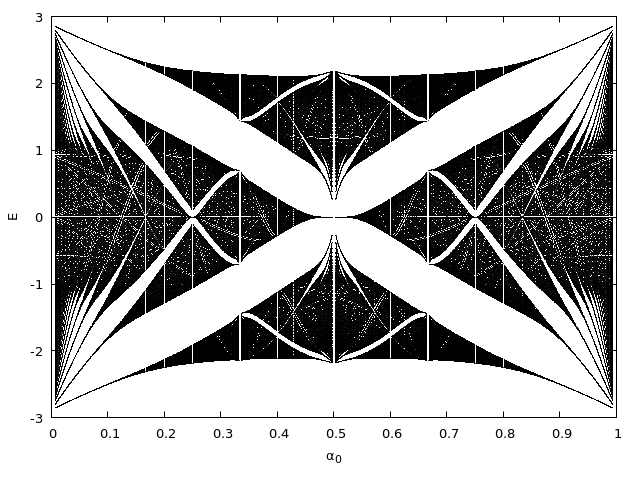
\includegraphics[width=\textwidth]{linear-spectrum}
\end{figure}
  \end{column}
  \begin{column}{0.5\textwidth}
      \begin{figure}[h]
 \centering
 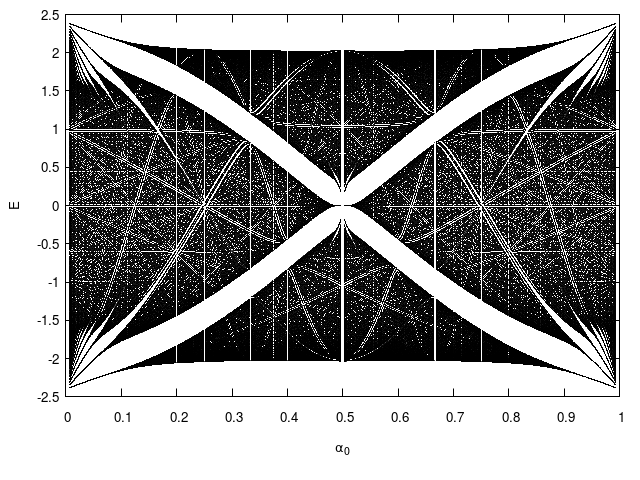
\includegraphics[width=\textwidth]{linear-spectrum5}
\end{figure}
  \end{column}
 \end{columns}
\end{frame}

\begin{frame}{Driven Aubry-Andr\'e-Harper Model}{Linearly Polarized Electric Field}
 \alert{Metal-Insulator transition}
 \begin{figure}[h]
  \centering
  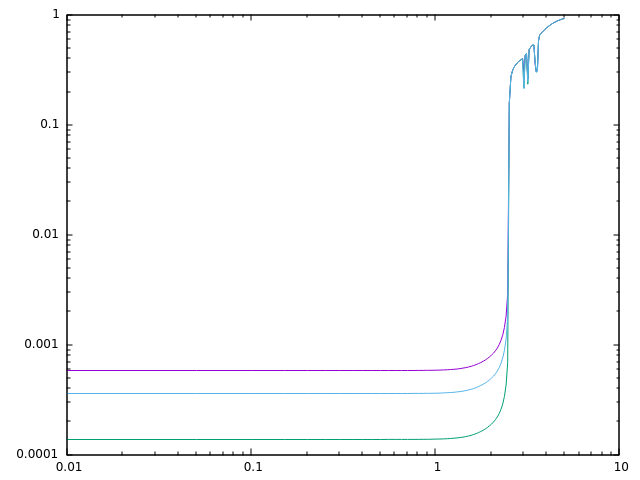
\includegraphics[width=0.6\textwidth]{ipr-linear}
 \end{figure}
\end{frame}

\begin{frame}{Driven Aubry-Andr\'e-Harper Model}{Linearly Polarized Electric Field}
\alert{Topological transitions}
 \begin{columns}
  \begin{column}{0.5\textwidth}
   \begin{figure}[h]
 \centering
 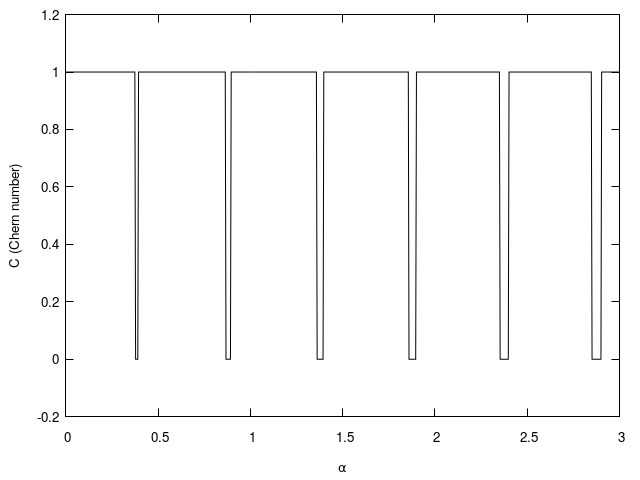
\includegraphics[width=\textwidth]{linear-chern-3a}
\end{figure}
  \end{column}
  \begin{column}{0.5\textwidth}
      \begin{figure}[h]
 \centering
 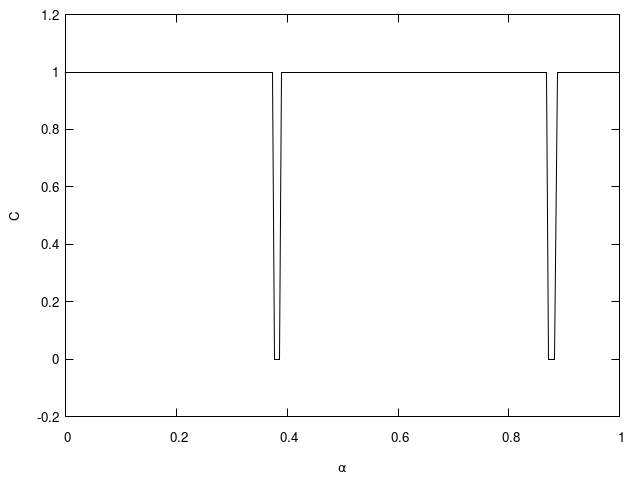
\includegraphics[width=\textwidth]{linear-chern-5a}
\end{figure}
  \end{column}
 \end{columns}
\end{frame}

\subsection{Circularly Polarized Light}
\begin{frame}{Driven Aubry-Andr\'e-Harper Model}{Circularly Polarized Electric Field}
As was the case for Linearly Polarized light, the Magnetic Translation Group is not affected by
Circularly Polarized Light. The model still retains the q-subband structure.

The momentum space Hamiltonian is
\begin{equation}
 \begin{split} H(k_x, k_y, t)_{i,j} = 
                   \delta_{i+1,j} + \delta_{i,j+1} + 2 \lambda \cos(k_y - 2\pi\alpha\sin{\omega t} + 2\pi\alpha_0 j)\delta_{i,j} \\
                   + \delta_{i,1}\delta_{j,q} e^{-i(k_x -2\pi\alpha\cos{\omega t})q}+\delta_{i,q}\delta_{j,1} e^{i(k_x -2\pi\alpha\cos{\omega t})q}
                  \end{split}
\end{equation}

Using BW perturbation we perturbatively obtain the effective Hamiltonian.
\end{frame}

\begin{frame}{Driven Aubry-Andr\'e-Harper Model}{Circularly Polarized Electric Field}
 \alert{Spectrum}
 \begin{figure}[h]
 \centering
 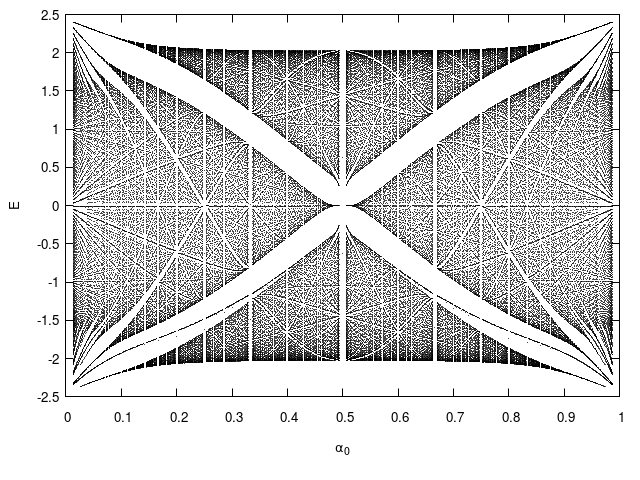
\includegraphics[width=0.7\textwidth]{cpl-spectrum} 
\end{figure}
\end{frame}

\begin{frame}{Driven Aubry-Andr\'e-Harper Model}{Circularly Polarized Electric Field}
 \alert{Topological Transitions}
  \begin{columns}
  \begin{column}{0.5\textwidth}
   \begin{figure}[h]
 \centering
 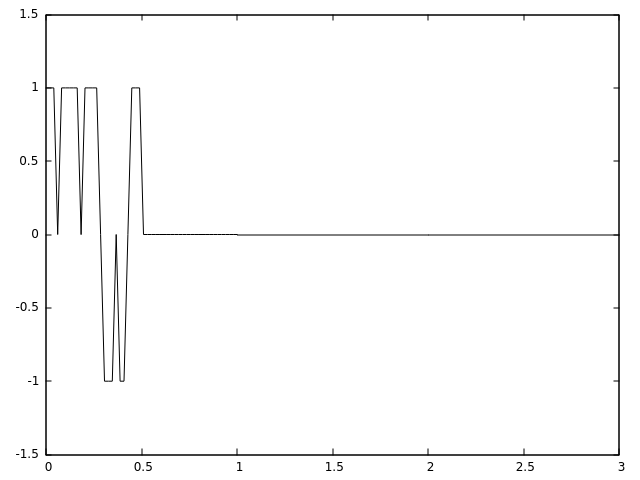
\includegraphics[width=\textwidth]{chern-band1}
\end{figure}
  \end{column}
  \begin{column}{0.5\textwidth}
      \begin{figure}[h]
 \centering
 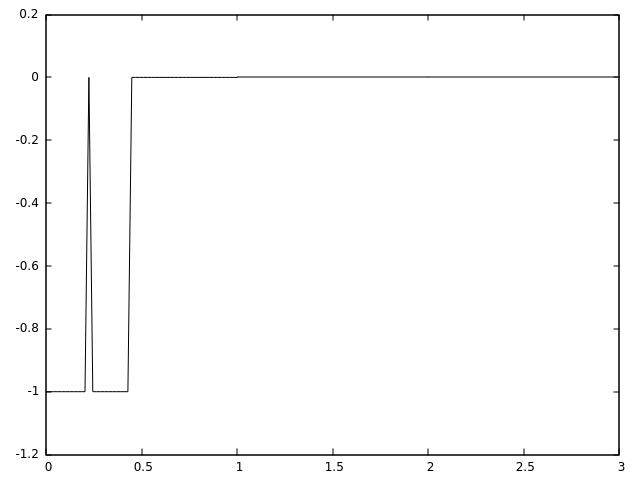
\includegraphics[width=\textwidth]{chern-band2}
\end{figure}
  \end{column}
 \end{columns}
\end{frame}


\section*{Summary}

\begin{frame}{Summary}
  \begin{itemize}\small
  \item
    Hall Conductivity is \alert{quantized}.
  \item
    Integral of Berry curvature over closed 2D surface is quantized - \alert{Chern numbers}.
  \item
    Chern numbers are related to Hall Conductivity.
  \item
    Floquet theory is a class of perturbation techniques used for time-periodic Hamiltonians.
  \item
    AAH Hamiltonian models electrons on 2D lattice under perpendicular uniform magnetic field.
  \item
    AAH model has a spectrum known as \alert{Hofstadter's butterfly}.
  \item
    AAH model has a metal-insulator phase transition.
  \item
    Hall conductivity of AAH model can be exactly determined.
  \item
    Oscillating Magnetic Field creates a mobility edge in the spectrum of AAH.
  \item
    Linearly polarized Electric field and Circularly polarized electric field driven models exhibit topological transitions.
  \end{itemize}  \normalsize
\end{frame}
\end{document}


